\documentclass{article}
\usepackage{pdfpages}
\title{Ph 20.1- Introduction to Python- Lissajous figures and beats}
\author{Stella Wang}
\date{17 January 2018}
\begin{document}
	\maketitle
\section{Lissajous curves}
We were first asked to investigate the relation between the ratio of fx/fy to the shape of the lissajous curve. All of the curves are closed when rational values are used. The when a higher ratio (fx/fy or fy/fx) used, more lobes and intersections were found in the resulting shape. Also whether fx $>$ fy or fx $<$ fy determined the orientation of the curve; whether it is rotated by 90 degrees or not. The following plots show the differences in the curves for fx/fy ratios of 1/9, 5/18, 3/5, 3/2, 3, 7/2 and 7/1.
\includepdf[pages={4,5,6,15,16,17,18}]{Week1plots.pdf}

Next, we investigated the effect of the phase shift $\phi$ on the shape of the curve when $fx=fy$. The phase shift has the effect of "tilting" the ellipse. It effectively rotates the curve and compresses it. It is notable that phase shifts of 0, $\pi$ and $2\pi$ produce the same curve, a circle, when everything else is held constant. This is helpful because if someone wants to perfectly align their circuit, they would want to see a circle on an oscilloscope. Otherwise, if they wished to tune it to a specific separation of phase, they could find the appropriate ellipse that corresponds to their desired phase shift. The following plots show the plots for phase shifts $\phi$ of 0, $\pi/10$, $\pi/4$, $\pi/2$, $2\pi/3$, $\pi$, $4\pi/3$ and $2\pi$.
\includepdf[pages={7,8,9,10,11,12,13,14}]{Week1plots.pdf}
 
 \section{Beats}
 Included are 3 plots that demonstrate the phenomenon of beats. The 3 plots correspond the frequencies of 377 and 383, 459 and 478 and 628 and 641. The frequency of the beats is calculated to be $\omega_1 - \omega_2$ because the waves the waves produced have two peaks of equal amplitude.
 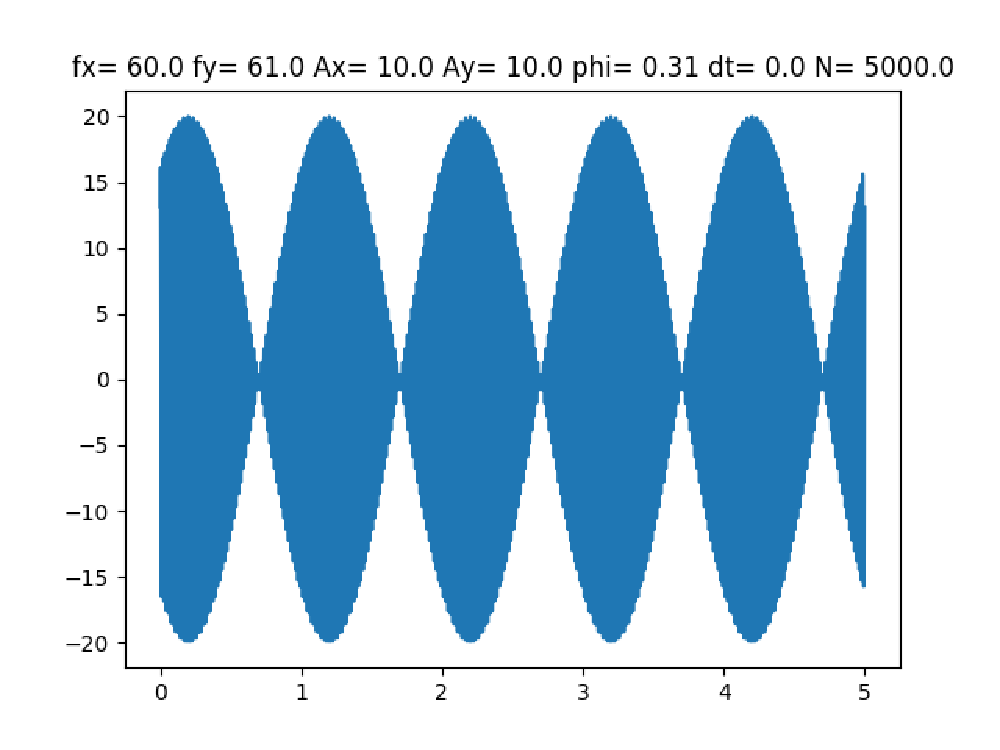
\includepdf[pages={1,2,3}]{Week1plots.pdf}
 
 \section{Conclusion}
 In this weeks assignment we used numpy arrays and lists to construct plots for Lissajous figures and beats. I have previously coded in python and used the numpy and matplotlib packages to do scientific analysis. This weeks assignment was helpful to review the Python language and the functions available in the numpy package. It was interesting to see the difference in computation speed between the numpy arrays and the for-loop-list method. I was previously advised to use numpy arrays for scientific computing but I had not entirely understood why. I now understand that the numpy array is a far more efficient data structure that compiles much easier and smoother than using the built in append function. 
 
This is the first \LaTeX  document that I have ever typed. While I am still working on learning the syntax and functions, I ultimately think this is a useful skill that I will hopefully improve at over the course of this term. For this assignment typing the \LaTeX  document turned out to be the most time consuming part. 

\end{document}